\documentclass[UTF8]{ctexart}
\usepackage{ctex}
\usepackage{amsthm,amsmath,amssymb}
\usepackage{color}
\usepackage[colorlinks,linkcolor=red]{hyperref}
\usepackage{mathrsfs}
\usepackage{boondox-cal}
\usepackage{braket}
\usepackage{graphicx}
\usepackage{epstopdf}
\usepackage{dutchcal}
\usepackage{lmodern}
\newcommand{\rank}{\mathrm{rank}}

\title{NewNET}
\author{}
\date{}
\pagestyle{plain}
\begin{document}
	\maketitle
    \section*{4 数据分析过程}
    \subsection*{预测方法的选择}
	\begin{align*}
		&\text{sequenceInputLayer(8)} \rightarrow \\
    	&\text{fullyConnectedLayer(300)} \rightarrow \\
    	&\text{reluLayer} \rightarrow \\
    	&\text{fullyConnectedLayer(300)} \rightarrow \\
    	&\text{reluLayer} \rightarrow \\
    	&\text{fullyConnectedLayer(300)} \rightarrow \\
    	&\text{reluLayer} \rightarrow \\
    	&\text{fullyConnectedLayer(numResponses)} \rightarrow \\
    	&\text{regressionLayer}
	\end{align*}
	注意到我们的数据集并不大, 这里搭建的网络也比较小, 这使得在个人电脑上进行训练成为可能.
    \subsection*{网络训练}
    首先, 我们从不同的类别中挑出几个有代表性的国家, 这里我们的选取是之前提到分类中的第二类的国家, 我们选取训练集为 France, South Korea, Australia, Canada, Iceland. 我们选取 Adam 优化器, 对上述数据训练 2000 个 epoches. 选取的用于验证的国家为 Saudi Arabia, Germany, Japan, United States. 初始的学习率设置为 $0.001$, 并每 75 个 epoch 乘以 $0.95$. 同样地, 定义一个 Kernel
	\[
	\mathcal{K} =
	\begin{bmatrix}
		\displaystyle\frac{1}{4}&\displaystyle\frac{1}{4}&\displaystyle\frac{1}{4}&\displaystyle\frac{1}{4}
	\end{bmatrix},
	\]
	我们将每日新增病例数与上面的核进行卷积, 考虑是两方面的: 一是为了方便网络的训练, 二是用四天的数据的平均来代替某一天的数据.
	\begin{figure}[htbp]
	    \centering
	    \subfigure{
	    \includegraphics[height=8cm, width=12cm]{regtrain.pdf}
	    }
	\end{figure}
	\subsection*{结果预测}
	我们将得到的网络用于预测中国和法国的新增病例数. 在得到的数据中, 我们将前 $\frac{4}{5}$ 的病例数作为训练集, 将后五分之一的数据作为测试集. 可以看到效果是很好的.
	\begin{figure}[htbp]
	    \centering
	    \subfigure{
	    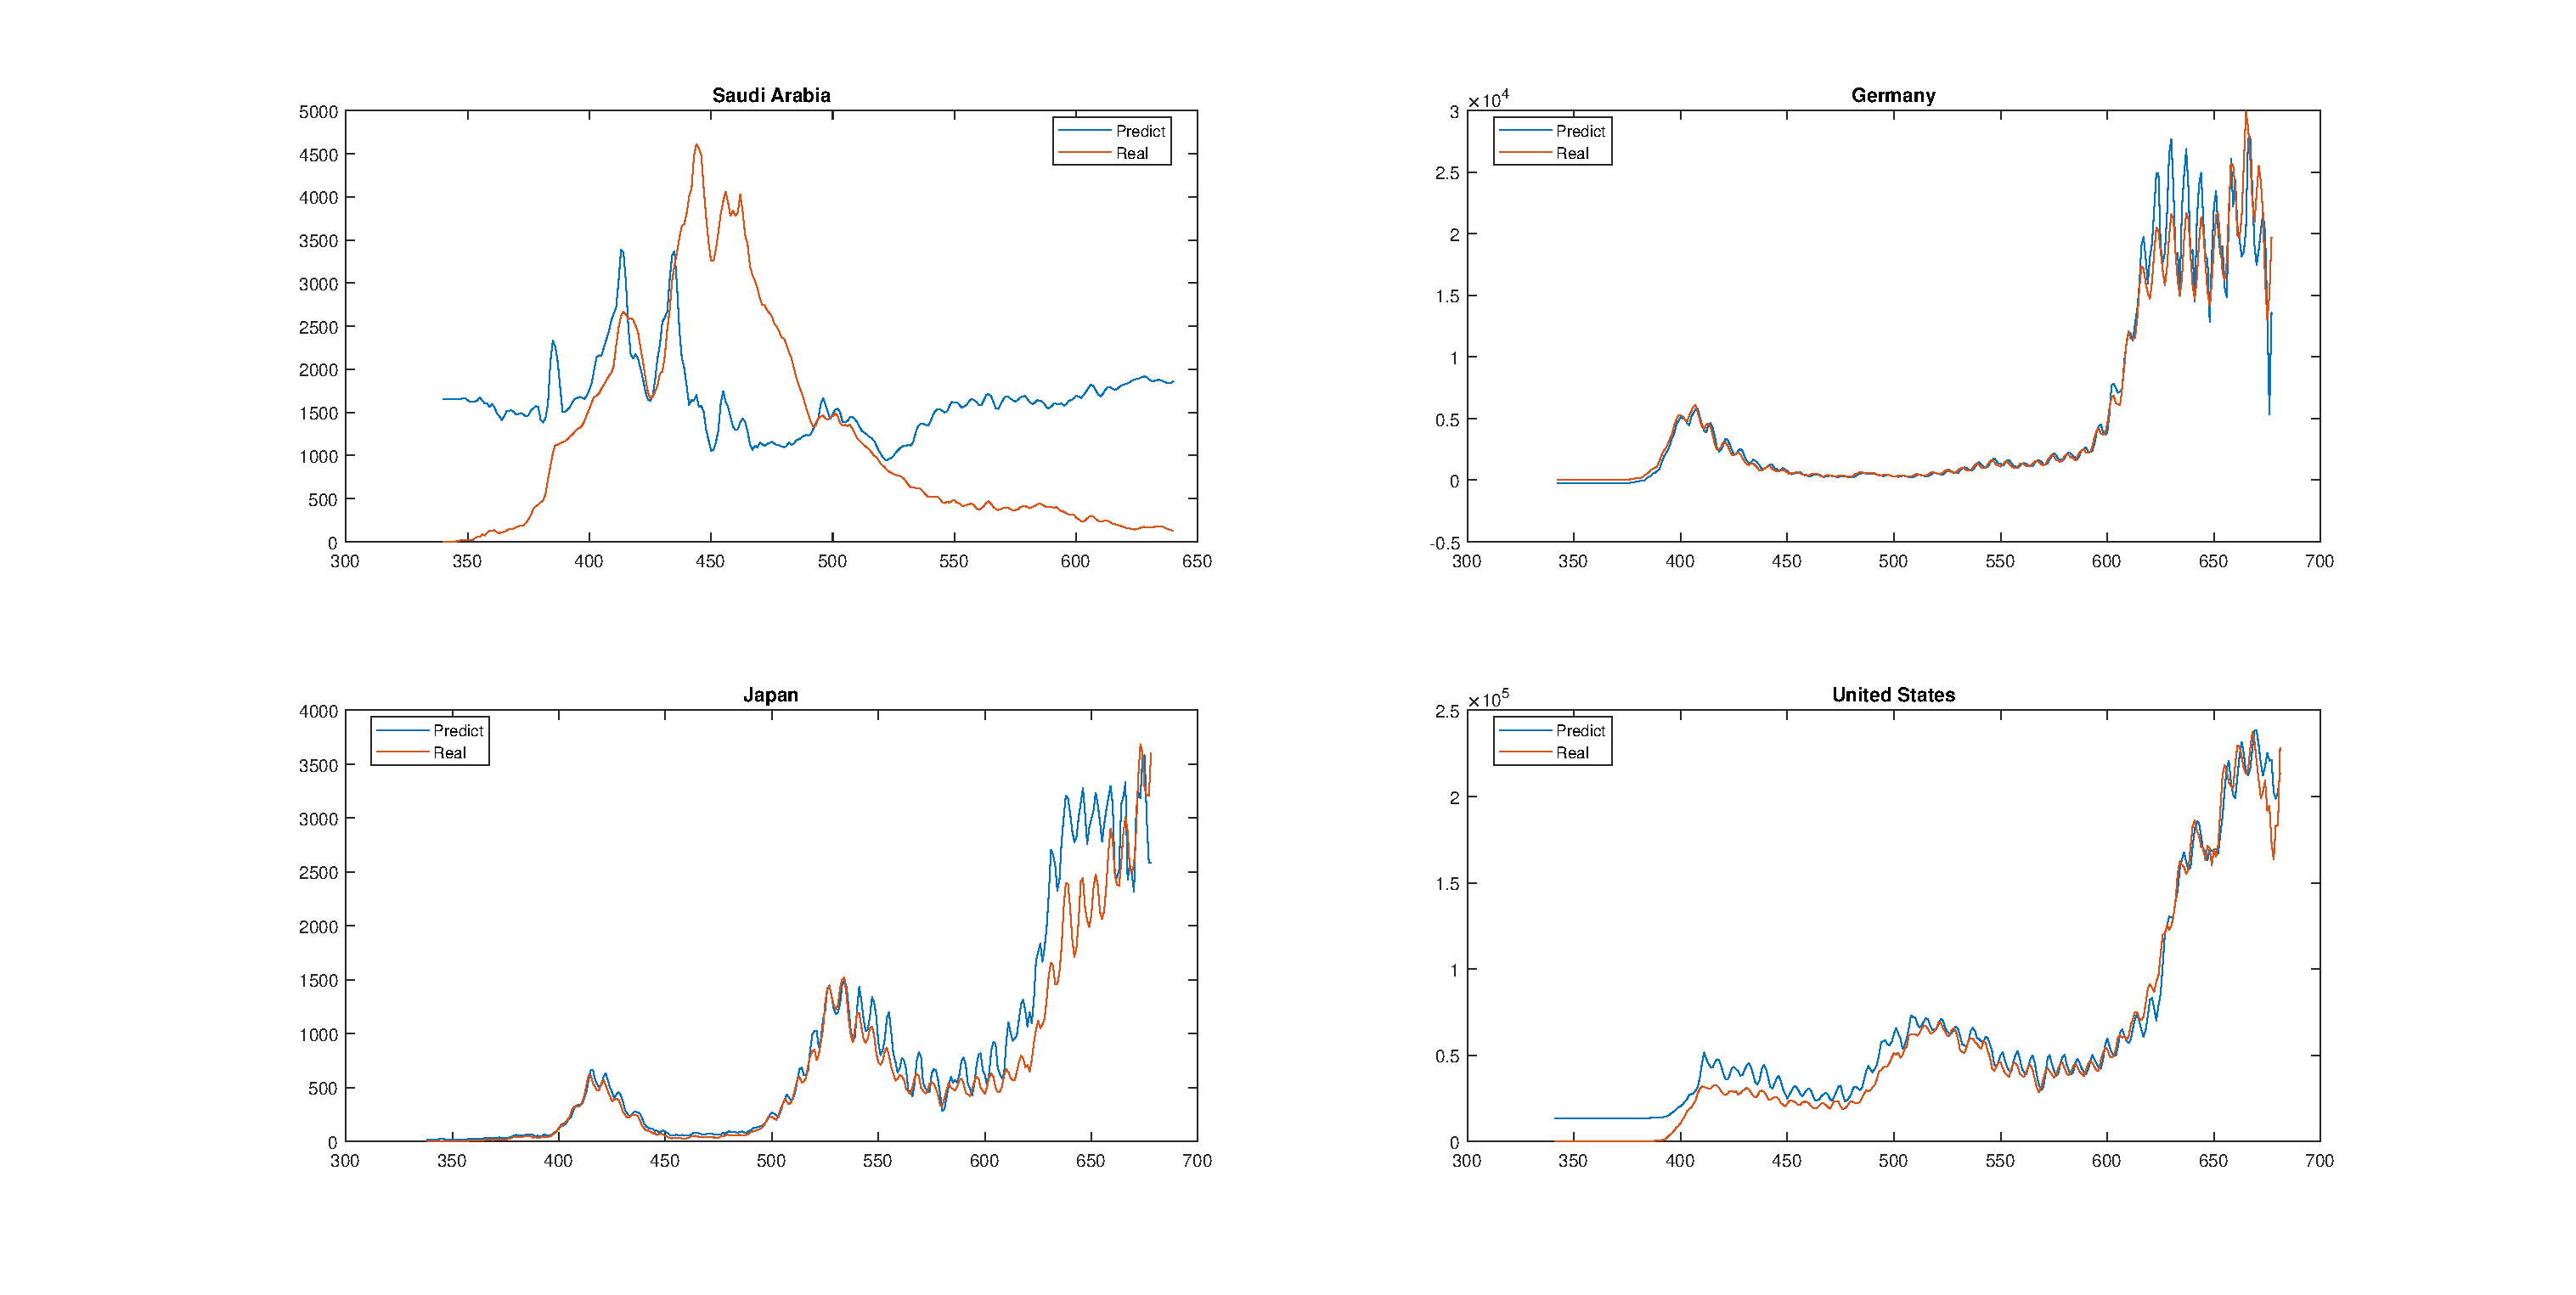
\includegraphics[height=12cm, width=14cm]{Pred2.eps}
	    }
	\end{figure}
    我们可以看到 Saudi Arabia 上, 我们的效果不好. 仔细观察我们可以发现, 这一国家的疫情形势也与其余三国不同. 所以我们可以认为我们的分类仍然存在一定的问题.
\end{document}
